%!TEX TS-program = xelatex
\documentclass[12pt, a4paper, oneside]{article}

\usepackage{amsmath,amsfonts,amssymb,amsthm,mathtools}  % пакеты для математики

\usepackage[english, russian]{babel} % выбор языка для документа
\usepackage[utf8]{inputenc} % задание utf8 кодировки исходного tex файла
\usepackage[X2,T2A]{fontenc}        % кодировка

\usepackage{fontspec}         % пакет для подгрузки шрифтов
\setmainfont{Linux Libertine O}   % задаёт основной шрифт документа

\usepackage{unicode-math}     % пакет для установки математического шрифта
\setmathfont[math-style=upright]{Neo Euler} % шрифт для математики

% Конкретный символ из конкретного шрифта
% \setmathfont[range=\int]{Neo Euler}

%%%%%%%%%% Работа с картинками %%%%%%%%%
\usepackage{graphicx}                  % Для вставки рисунков
\usepackage{graphics}
\graphicspath{{images/}{pictures/}}    % можно указать папки с картинками
\usepackage{wrapfig}                   % Обтекание рисунков и таблиц текстом

%%%%%%%%%%%%%%%%%%%%%%%% Графики и рисование %%%%%%%%%%%%%%%%%%%%%%%%%%%%%%%%%
\usepackage{tikz, pgfplots}  % язык для рисования графики из latex'a

%%%%%%%%%% Гиперссылки %%%%%%%%%%
\usepackage{xcolor}              % разные цвета

\usepackage{hyperref}
\hypersetup{
	unicode=true,           % позволяет использовать юникодные символы
	colorlinks=true,       	% true - цветные ссылки, false - ссылки в рамках
	urlcolor=blue,          % цвет ссылки на url
	linkcolor=black,          % внутренние ссылки
	citecolor=green,        % на библиографию
	pdfnewwindow=true,      % при щелчке в pdf на ссылку откроется новый pdf
	breaklinks              % если ссылка не умещается в одну строку, разбивать ли ее на две части?
}


\usepackage{todonotes} % для вставки в документ заметок о том, что осталось сделать
% \todo{Здесь надо коэффициенты исправить}
% \missingfigure{Здесь будет Последний день Помпеи}
% \listoftodos --- печатает все поставленные \todo'шки

\usepackage[paper=a4paper, top=20mm, bottom=15mm,left=20mm,right=15mm]{geometry}
\usepackage{indentfirst}       % установка отступа в первом абзаце главы

\usepackage{setspace}
\setlength{\parskip}{4mm}   % Расстояние между абзацами
% Разные длины в латехе https://en.wikibooks.org/wiki/LaTeX/Lengths


\usepackage{xcolor} % Enabling mixing colors and color's call by 'svgnames'

\definecolor{MyColor1}{rgb}{0.2,0.4,0.6} %mix personal color
\newcommand{\textb}{\color{Black} \usefont{OT1}{lmss}{m}{n}}
\newcommand{\blue}{\color{MyColor1} \usefont{OT1}{lmss}{m}{n}}
\newcommand{\blueb}{\color{MyColor1} \usefont{OT1}{lmss}{b}{n}}
\newcommand{\red}{\color{LightCoral} \usefont{OT1}{lmss}{m}{n}}
\newcommand{\green}{\color{Turquoise} \usefont{OT1}{lmss}{m}{n}}

\usepackage{titlesec}
\usepackage{sectsty}
%%%%%%%%%%%%%%%%%%%%%%%%
%set section/subsections HEADINGS font and color
\sectionfont{\color{MyColor1}}  % sets colour of sections
\subsectionfont{\color{MyColor1}}  % sets colour of sections

%set section enumerator to arabic number (see footnotes markings alternatives)
\renewcommand\thesection{\arabic{section}.} %define sections numbering
\renewcommand\thesubsection{\thesection\arabic{subsection}} %subsec.num.

%define new section style
\newcommand{\mysection}{
	\titleformat{\section} [runin] {\usefont{OT1}{lmss}{b}{n}\color{MyColor1}} 
	{\thesection} {3pt} {} } 


%	CAPTIONS
\usepackage{caption}
\usepackage{subcaption}
%%%%%%%%%%%%%%%%%%%%%%%%
\captionsetup[figure]{labelfont={color=Turquoise}}

\pagestyle{empty}

%%%%%%%%%% Свои команды %%%%%%%%%%
\usepackage{etoolbox}    % логические операторы для своих макросов

% Все свои команды лучше всего определять не по ходу текста, как это сделано в этом документе, а в преамбуле!

% Одно из применений - уничтожение какого-то куска текста!
\newbool{answers}
\booltrue{answers}
%\boolfalse{answers}

\usepackage{enumitem}
% бульпоинты в списках
\definecolor{myblue}{rgb}{0, 0.45, 0.70}
\newcommand*{\MyPoint}{\tikz \draw [baseline, fill=myblue,draw=blue] circle (2.5pt);}
\renewcommand{\labelitemi}{\MyPoint}

% расстояние в списках
\setlist[itemize]{parsep=0.4em,itemsep=0em,topsep=0ex}
\setlist[enumerate]{parsep=0.4em,itemsep=0em,topsep=0ex}


\title{Все любят пиццу}
\author{Большое домашнее задание по курсу <<Введение в анализ данных>> № 2}
\date{1 июня 2019 г.}

\begin{document}

\maketitle

\section{Общая постановка задания}

Мистер Пануччи владеет сетью пиццерий. Для доставки пиццы мистер Пануччи использует довольно большую сеть из курьеров. Он, как  мудрый менеджер, понимает, что его текущая система работает неоптимально. В одних районах курьеры регулярно простаивают, в других не хватает рук, и заказы опаздывают. Хочется с помощью машинного обучения решить эту проблему, и каждую неделю перераспределять силы курьеров так, чтобы они не простаивали, и все заказчики получали свою пиццу вовремя. 

Вам предлагается подумать о том, как эту проблему можно было бы решить. Для того, чтобы решить эту задачу, вам нужно ответить на следущую серию вопросов: 


\begin{enumerate} 
	\item Как можно измерить, сколько денег сейчас теряет мистер Пануччи из-за неоптимальности курьерской сети? 
	\item \textbf{Какую именно целевую переменную надо научиться прогнозировать}, чтобы решить проблемы, связанные с курьерами? \textbf{Что за задачу машинного обучения  придётся для этого решить} (классификация/регрессия и тп) ?
	\item Как надо использовать прогнозы, чтобы решить проблемы пиццерии? Чтобы ответить на этот пункт, нужно описать схему того, как ваши прогнозы помогают оптимально распределить курьеров по районам.
    \item \textbf{Какие переменные можно было бы использовать в качестве объясняющих?} Откуда их взять (попробуйте отобрать те переменные, которые реально раздобыть)?
    \item Какие этапы предобработки нужно провести с данными перед тем, как обучать для них модель? С какими проблемами вы скорее всего столкнётесь (переобучение, выбросы, пропуски и другое)? Как вы будете с ними бороться? 
    \item \textbf{Как можно измерить пользу от внедрения новой системы распределения курьеров?} 
\end{enumerate}

На выходе должен получиться небольшой текст, в котором находятся ваши рассуждения. Пожалуйста, структурируйте их так, чтобы было понятно где и на какие вопросы вы отвечаете. \textbf{Внимание!}  Не надо писать огромный мануал про машинное обучение! Постарайтесь изложить все свои мысли на 2-3 страницах \textbf{структурированного понятного текста.}  Работа сдаётся в формате pdf в anytask. 

\newpage 

\section{Организационные мелочи} 

\subsection*{Команды}

Задание  выполняется в командах по 2-3 человека. Индивидуальные работы не будут засчитаны.

\subsection*{Дедлайн}

\begin{itemize}
\item Задание выдаем 04.06.2019
\item Задание сдаем 13.06.2019 в 23.30 на \url{anytask.org}
\end{itemize} 

\subsection*{В каком виде сдаём?} 

\begin{enumerate}
	\item  Ждем ваши мысли в виде pdf-ки
	\item  Пожалуйста, укажите в своей работе всех членов команды и номер группы. 
    \item  Постарайтесь делать осмысленные выводы! Не будьте мудрыми, как король: 
		
		\begin{center}
			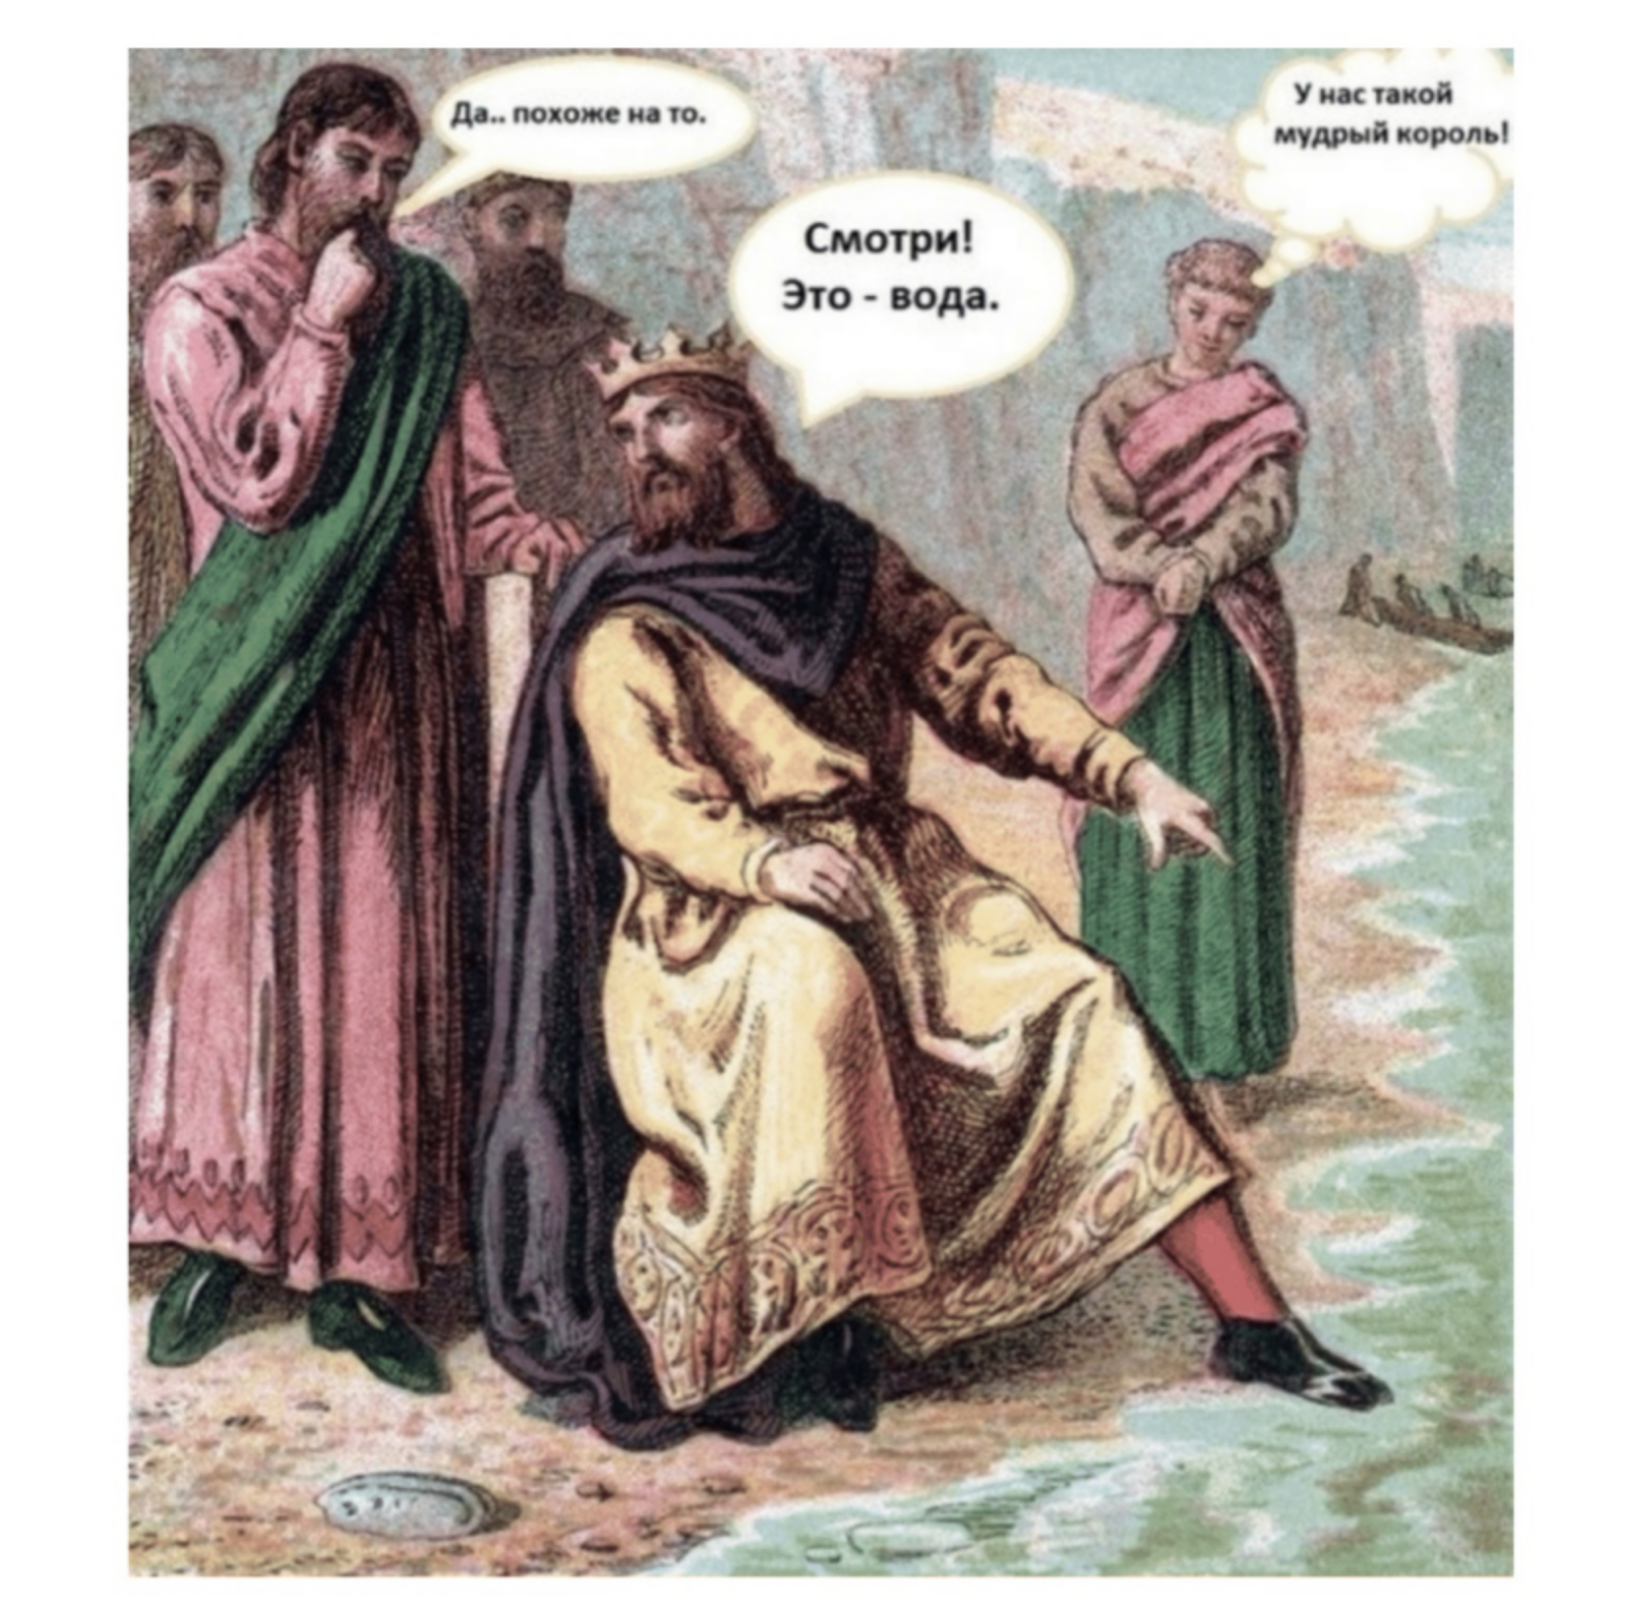
\includegraphics[scale=0.2]{laba_1.png}
		\end{center}
	
\end{enumerate}

\subsection*{Оценивание}

Работа оценивается по $10$-бальной шкале.  Она ставится на команду и нормируется на число человек в ней. Так, если в команде три человека и она получает оценку $8$, она превращается в $24$ балла. Далее участники команды делят эти баллы между собой в любой пропорции в зависимости от вклада каждого участника в итоговую работу. Если в команде два участника, то $8$ соотвественно превращается в $16$.  

Ваша итоговая оценка зависит от того, насколько глубоко проработана задача, насколько чётко обоснован каждый этап работы, каждая метрика.  



\end{document}
